\section{Data and Exploratory Analysis}

Before modeling the data, we did an exploratory data analysis that is an initial visualization and decomposition of the data to understand its underlying structure, including trend and seasonality. We also divided the data into training and testing sets.
After that, we applied some data transformation to stabilize the variance and stationarize the series.\

\subsection{Dataset Description}
The analysed data was obtained from the Eurostat portal \cite{EurostatElectricityConsumption}. The dataset refers to the monthly amount of electricity available on the domestic market in France, expressed in gigawatt hours (GWh).
The data is updated monthly and covers the period from January 2008 to March 2025, comprising 207 months of observations.
The selected indicator is 'Electricity available for the internal market – monthly data (France)'.

This type of series is particularly relevant for studying energy consumption patterns over time, including seasonal variations and structural trends.

The dataset was imported from a .csv file to create a time series object with a monthly frequency starting in January 2008.

\subsection{Separation into training and testing sets}

To properly assess the models' predictive capacity, the data was divided as follows:

- Training: 80\% of the initial observations (January 2008 – October 2021), 165 observations.

- Test: the remaining 20\% (November 2021 – March 2025), 42 observations.

We only applied transformations to the training set (repeating this process in the test set when necessary) to avoid data leakage.

\subsection{Exploratory Analysis}

To study the existence of outliers, we used a box plot, Fig.\ref{fig:bx-plot}, treating the numerical values by replacing commas with decimal points. We observed that the boxplot indicates the absence of outliers.

\begin{figure}[H]
    \centering
    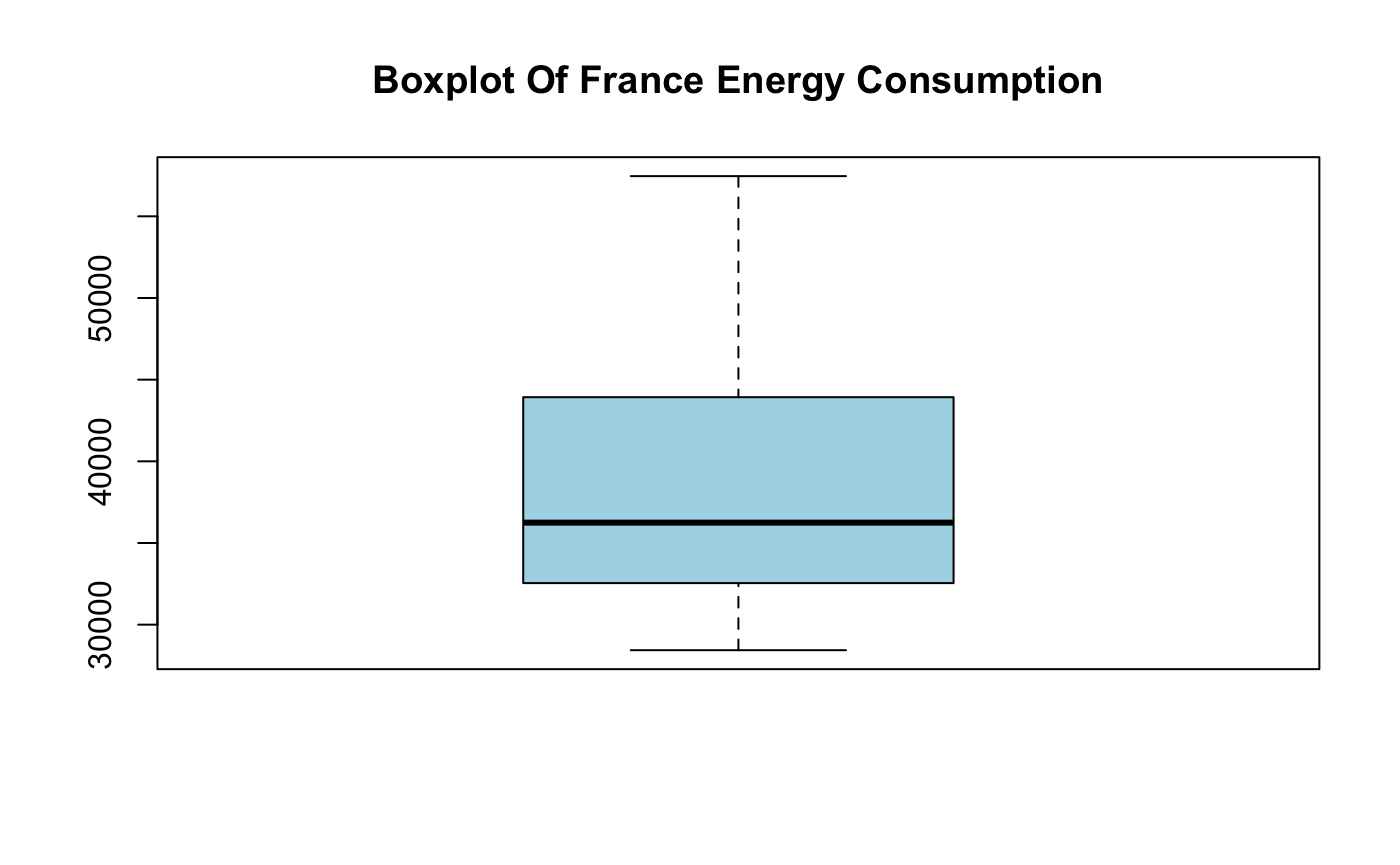
\includegraphics[width=0.75\linewidth]{images/box-plot.png}
    \caption{Box-Plot of Energy Consumption in France}
    \label{fig:bx-plot}
\end{figure}

To identify visual patterns we visualizes the time series using a plot, Fig\ref{fig:f-plot}. 
\begin{figure}[H]
    \centering
    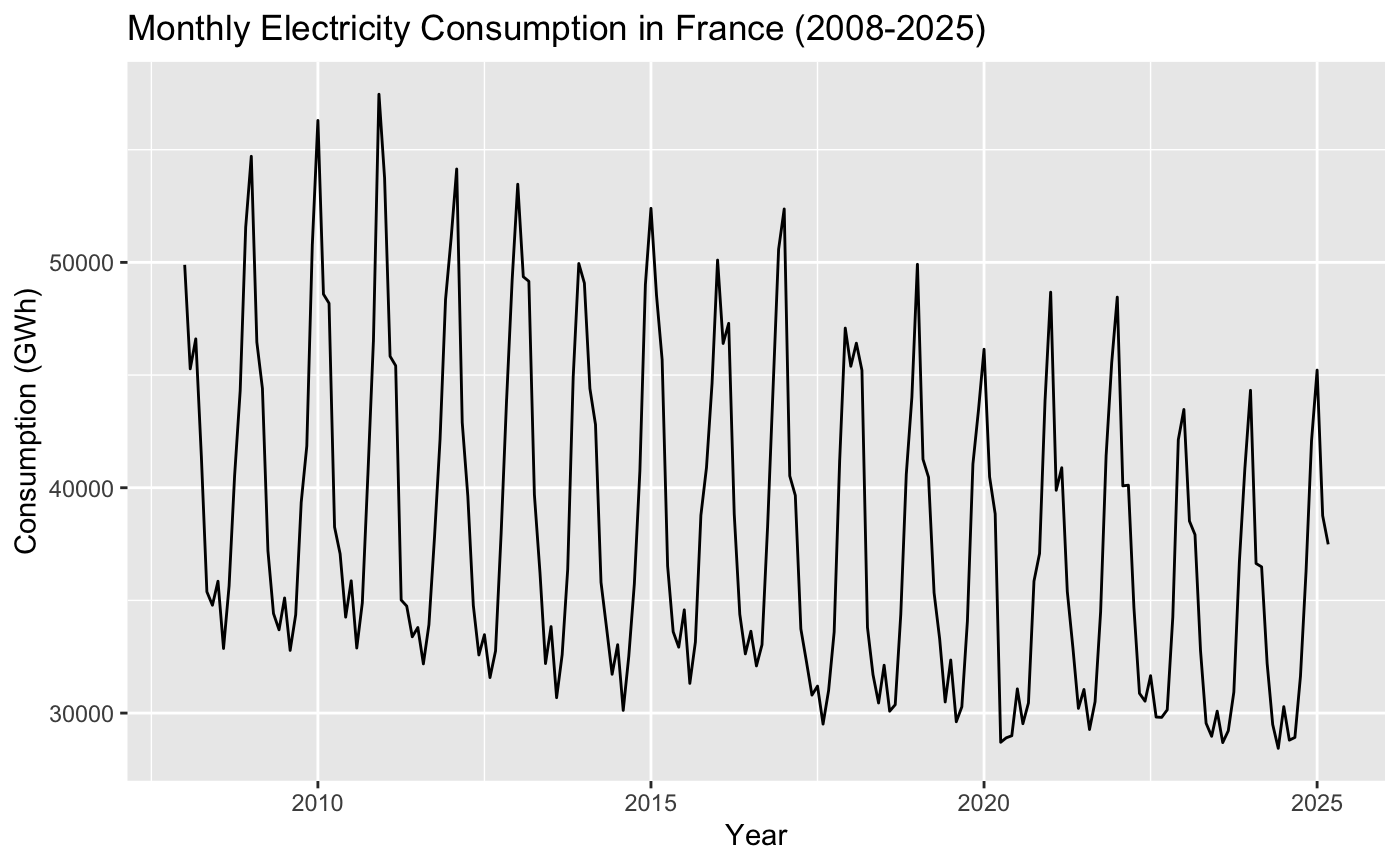
\includegraphics[width=0.75\linewidth]{images/f-plot.png}
    \caption{Monthly Electricity Consumption in France (2008-2025)}
    \label{fig:f-plot}
\end{figure}
We concluded that the time series has:
\begin{itemize}
    \item Strong seasonality: there are regular peaks in the winter months and lows in the summer months.
    \item Slightly decreasing trend: especially since 2010.
    \item Slight variation in variance: the level of consumption shows greater variability in the early years, which seems to decrease slightly over time.
\end{itemize}

\vspace{0.5\baselineskip}


We also decomposed the time series to better visualize these components (trend, seasonality and noise) and prove our last conclusions, Fig.\ref{fig:f2}.
We applied classical decomposition since our data has clear and stable trend and sazonality.

The decomposition confirms the strong seasonal pattern and a visible, though slightly noisy, trend that becomes evident especially after 2010.

\begin{figure}[H]
    \centering
    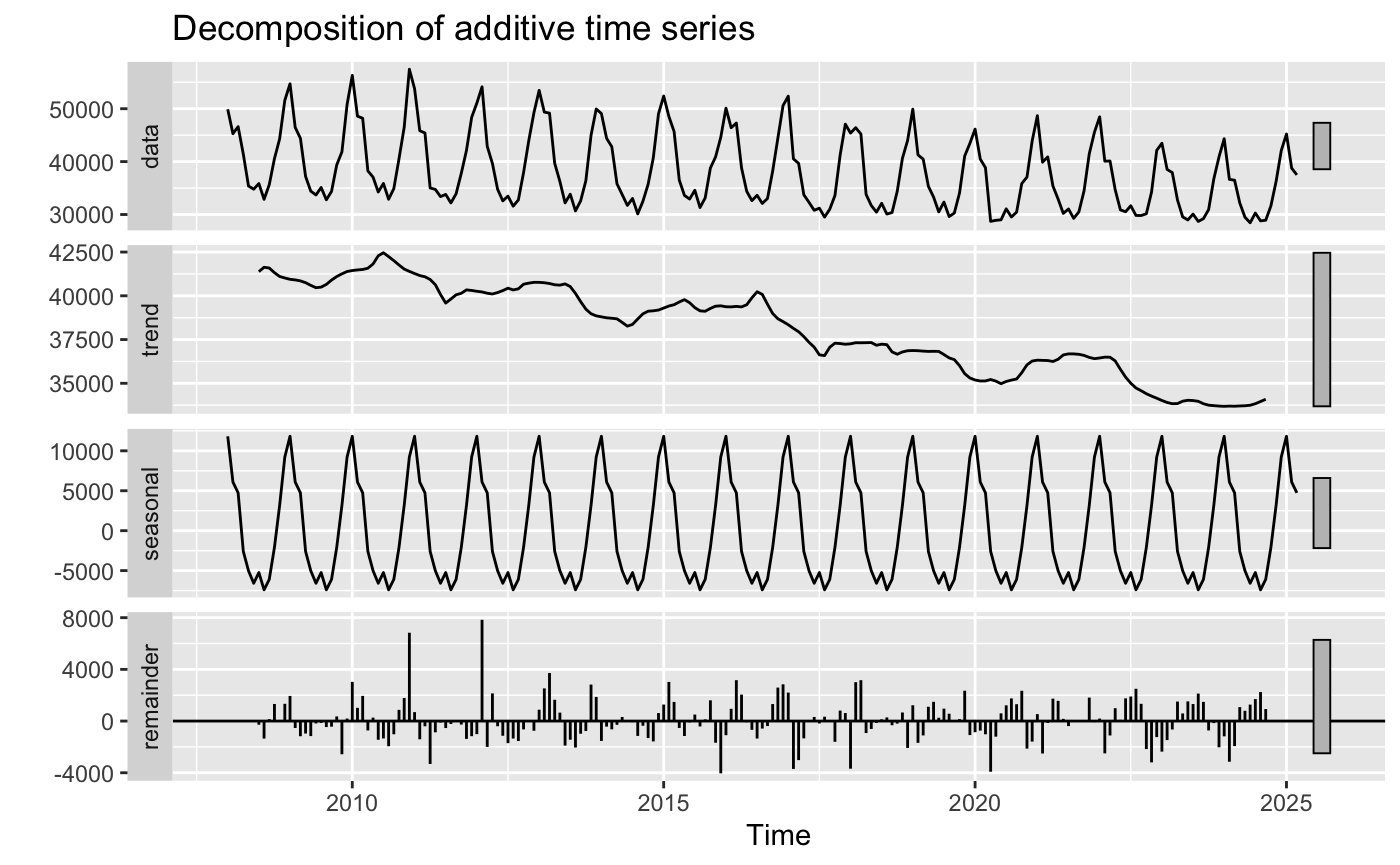
\includegraphics[width=1\linewidth]{images/f2.png}
    \caption{Time Series Decomposition}
    \label{fig:f2}
\end{figure}

The characteristics of the series, seasonality and trend, suggest the need for models such as SARIMA, ETS or STL + ARIMA decomposition, that will be explored in the following sections.

\subsection{Data Transformations}
Following the initial exploratory analysis, we confirmed that the time series exhibited variations in variance and trend fluctuations. To address this, we need to apply some transformations.

\subsubsection{Stabilise Variance}

\vspace{0.5\baselineskip}

To stabilise the variance of the time series, we applied a logarithmic transformation, Fig.\ref{fig:log}
A visual inspection of the original series indicates greater seasonal fluctuations during periods of higher consumption, notably between 2008 and 2012, and less pronounced variation in subsequent years.
This pattern indicates that the variance is not constant and may depend on the level of the series, a condition known as heteroscedasticity.

Applying the log() transformation reduces this heteroscedasticity, making the series more suitable for modelling, particularly for models that assume constant variance.

\begin{figure}[H]
    \centering
    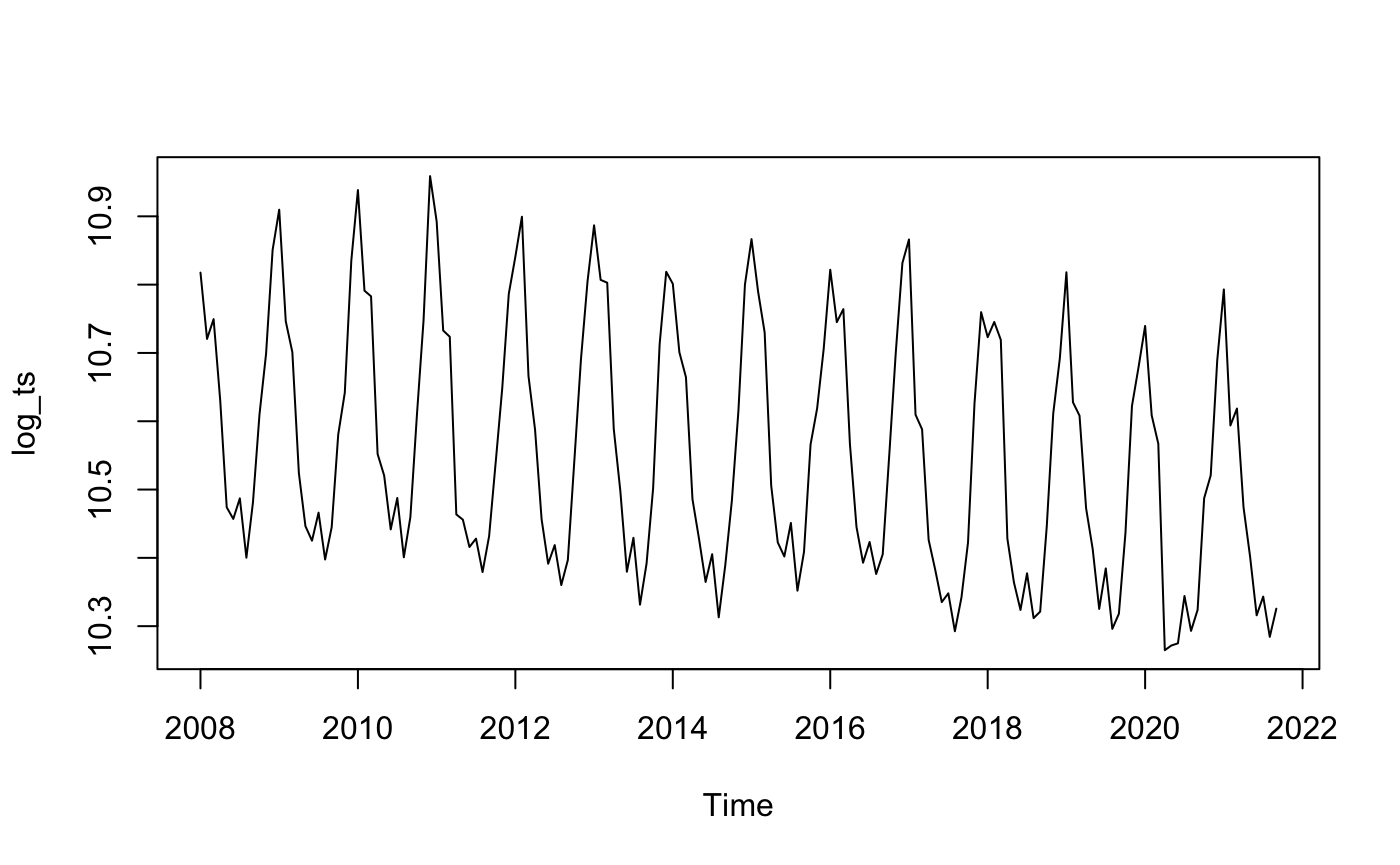
\includegraphics[width=0.9\linewidth]{images/log.png}
    \caption{Time Series Log Transformation}
    \label{fig:log}
\end{figure}


\subsubsection{Stationarity Testing and Differencing}

\vspace{0.5\baselineskip}

For the conclusions of the exploratory analysis we already known that the trend was not constant just by observing the time series plot. However, to rich this paper, we did some formal stationarity tests with ADF and KPSS to check if we do need to differenciate the time series. We can confirm this with statistical tests.

We applied two complementary tests:
\begin{itemize}
    \item Augmented Dickey-Fuller (ADF) test:
    \begin{center}
        \( H_0: \text{The series is non-stationary (has a unit root).} \)
    \end{center}
    \item KPSS test:
    \begin{center}
        \( H_0: \text{The series is stationary.} \)
    \end{center}
\end{itemize}

\vspace{0.5\baselineskip}

For both tests, a low p-value (less than 0.05) means that we can reject the null hypothesis (H0).
However, as the results were ambiguous, it is safer to differentiate the series, assuming that it is not yet fully stationary.

\vspace{0.5\baselineskip}

To determine the order of differencing we used the functions \textit{ndiffs()} for regular differencing and \textit{nsdiffs()} for seasonal differencing. The results were 1 for each differencing.

\begin{figure}[H]
    \centering
    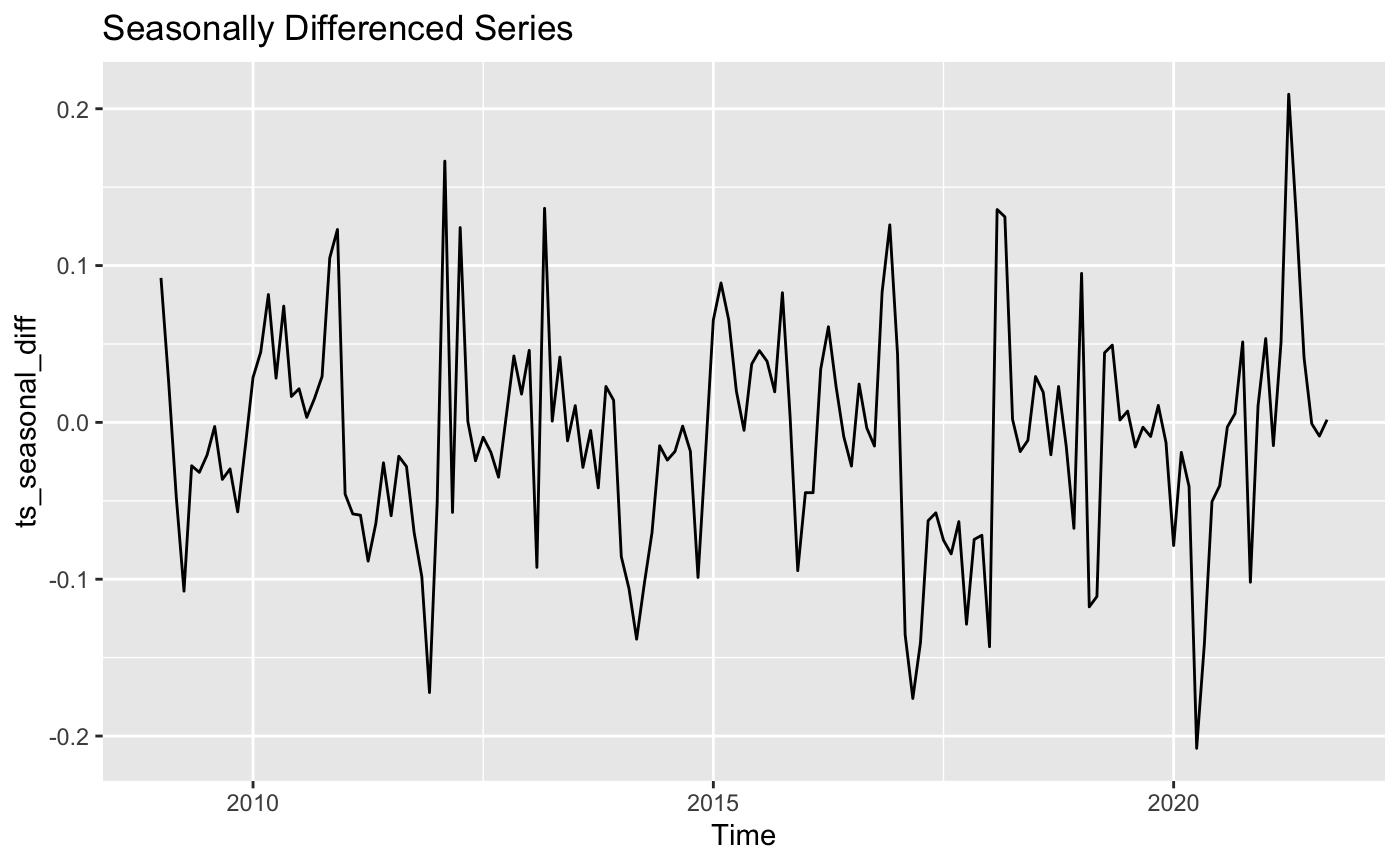
\includegraphics[width=0.9\linewidth]{images/seasonali_diff.png}
    \caption{Seasonally Differenced Series ((D=1)}
    \label{fig:seasonali_diff}
\end{figure}

For this reason, we started with seasonal differencing, Fig.\ref{fig:seasonali_diff}, (lag = 12) due to the strong 12-month seasonality.
Although the seasonal pattern has now disappeared, there may still be a trend present, so we applied a regular first difference to remove any remaining trend, Fig.\ref{fig:seasonaly_regulary}.

\begin{figure}[H]
    \centering
    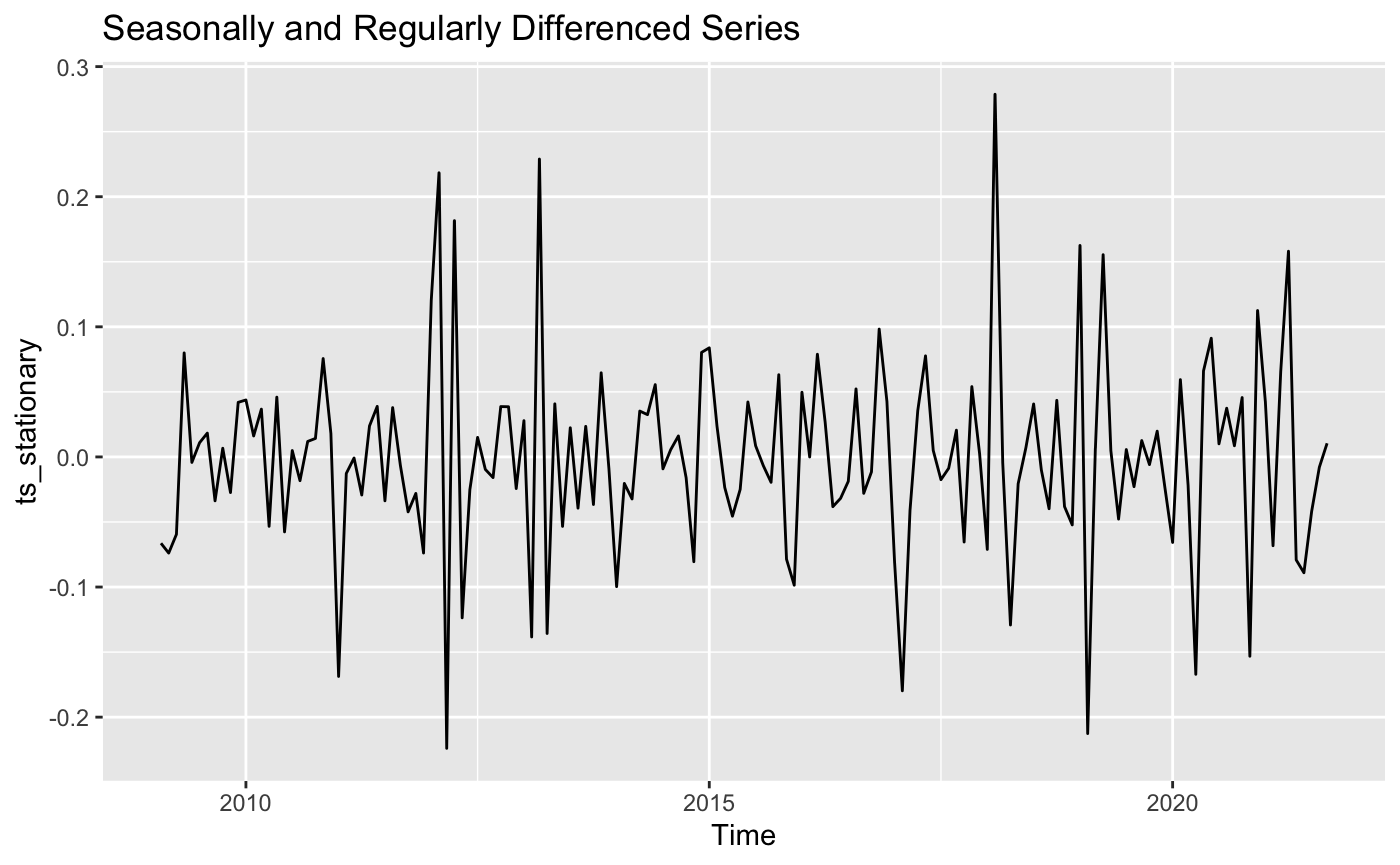
\includegraphics[width=0.9\linewidth]{images/seasonaly_regulary.png}
    \caption{Seasonally and Regularly Differenced Series(d=1)}
    \label{fig:seasonaly_regulary}
\end{figure}


To confirm the stationarity of the time series after differencing, we re-ran the stationarity tests (ADF and KPSS). Both tests then agreed on the stationarity of the time series. The Augmented Dickey-Fuller (ADF) test strongly rejected the null hypothesis of non-stationarity ($p < 0.01$), while the KPSS test failed to reject the null hypothesis of stationarity ($p > 0.1$). These results confirmed that the differenced series was stationary.